\section{Results}
\label{sec:results}

\para{Main comparison.} \Tabref{tab:main_results} reports the core results. The strongest text-only result appears in \longterm: \gptmodel improves mean \brier from 0.200 for the crowd to 0.151 and raises accuracy from 0.600 to 0.767. The same prompt fails in \shortterm, where the crowd remains much better with \brier 0.065 versus 0.131 for the model. This reversal is important because it rejects the broad claim that a single text-only LLM forecast dominates the crowd in both regimes.

\para{Effect of historical crowd trajectories.} Adding structured crowd history has opposite effects across regimes. In \shortterm, it sharply improves the model from 0.131 to 0.056 \brier, narrowly beating the crowd's 0.065 and raising accuracy from 0.833 to 0.933. In \longterm, the same addition worsens the model from 0.151 to 0.174 \brier. This pattern suggests that late-stage dense questions benefit from explicit temporal human signal, while early sparse questions may be harmed by anchoring to a thin or noisy trajectory.

\para{Statistical tests.} \Tabref{tab:paired_tests} shows the paired analysis. None of the four LLM-versus-crowd comparisons reach $p < 0.05$. The most favorable mean paired difference is $-0.050$ in \longterm under \questiononly, but its 95\% confidence interval $[-0.143, 0.037]$ crosses zero. The least favorable is $+0.066$ in \shortterm under \questiononly, with confidence interval $[-0.012, 0.154]$. We therefore interpret direction, magnitude, and consistency across conditions as suggestive evidence rather than proof of superiority.

\begin{table*}[t]
\centering
\caption{Main forecasting results by regime and prompt condition. Lower \brier is better. Best LLM-or-crowd result within each row is shown in \textbf{bold}.}
\label{tab:main_results}
\resizebox{\textwidth}{!}{%
\begin{tabular}{@{}llccccccc@{}}
\toprule
Regime & Prompt & $n$ & LLM \brier & Crowd \brier & 0.5 Baseline & LLM Acc. & Crowd Acc. & Mean Diff. \\
\midrule
\longterm & \questiononly & 30 & {\bf 0.151} & 0.200 & 0.250 & {\bf 0.767} & 0.600 & -0.050 \\
\longterm & \withhistory & 30 & {\bf 0.174} & 0.200 & 0.250 & {\bf 0.633} & 0.600 & -0.026 \\
\shortterm & \questiononly & 30 & 0.131 & {\bf 0.065} & 0.250 & 0.833 & {\bf 0.900} & +0.066 \\
\shortterm & \withhistory & 30 & {\bf 0.056} & 0.065 & 0.250 & {\bf 0.933} & 0.900 & -0.010 \\
\bottomrule
\end{tabular}%
}
\end{table*}



\begin{figure}[t]
    \centering
    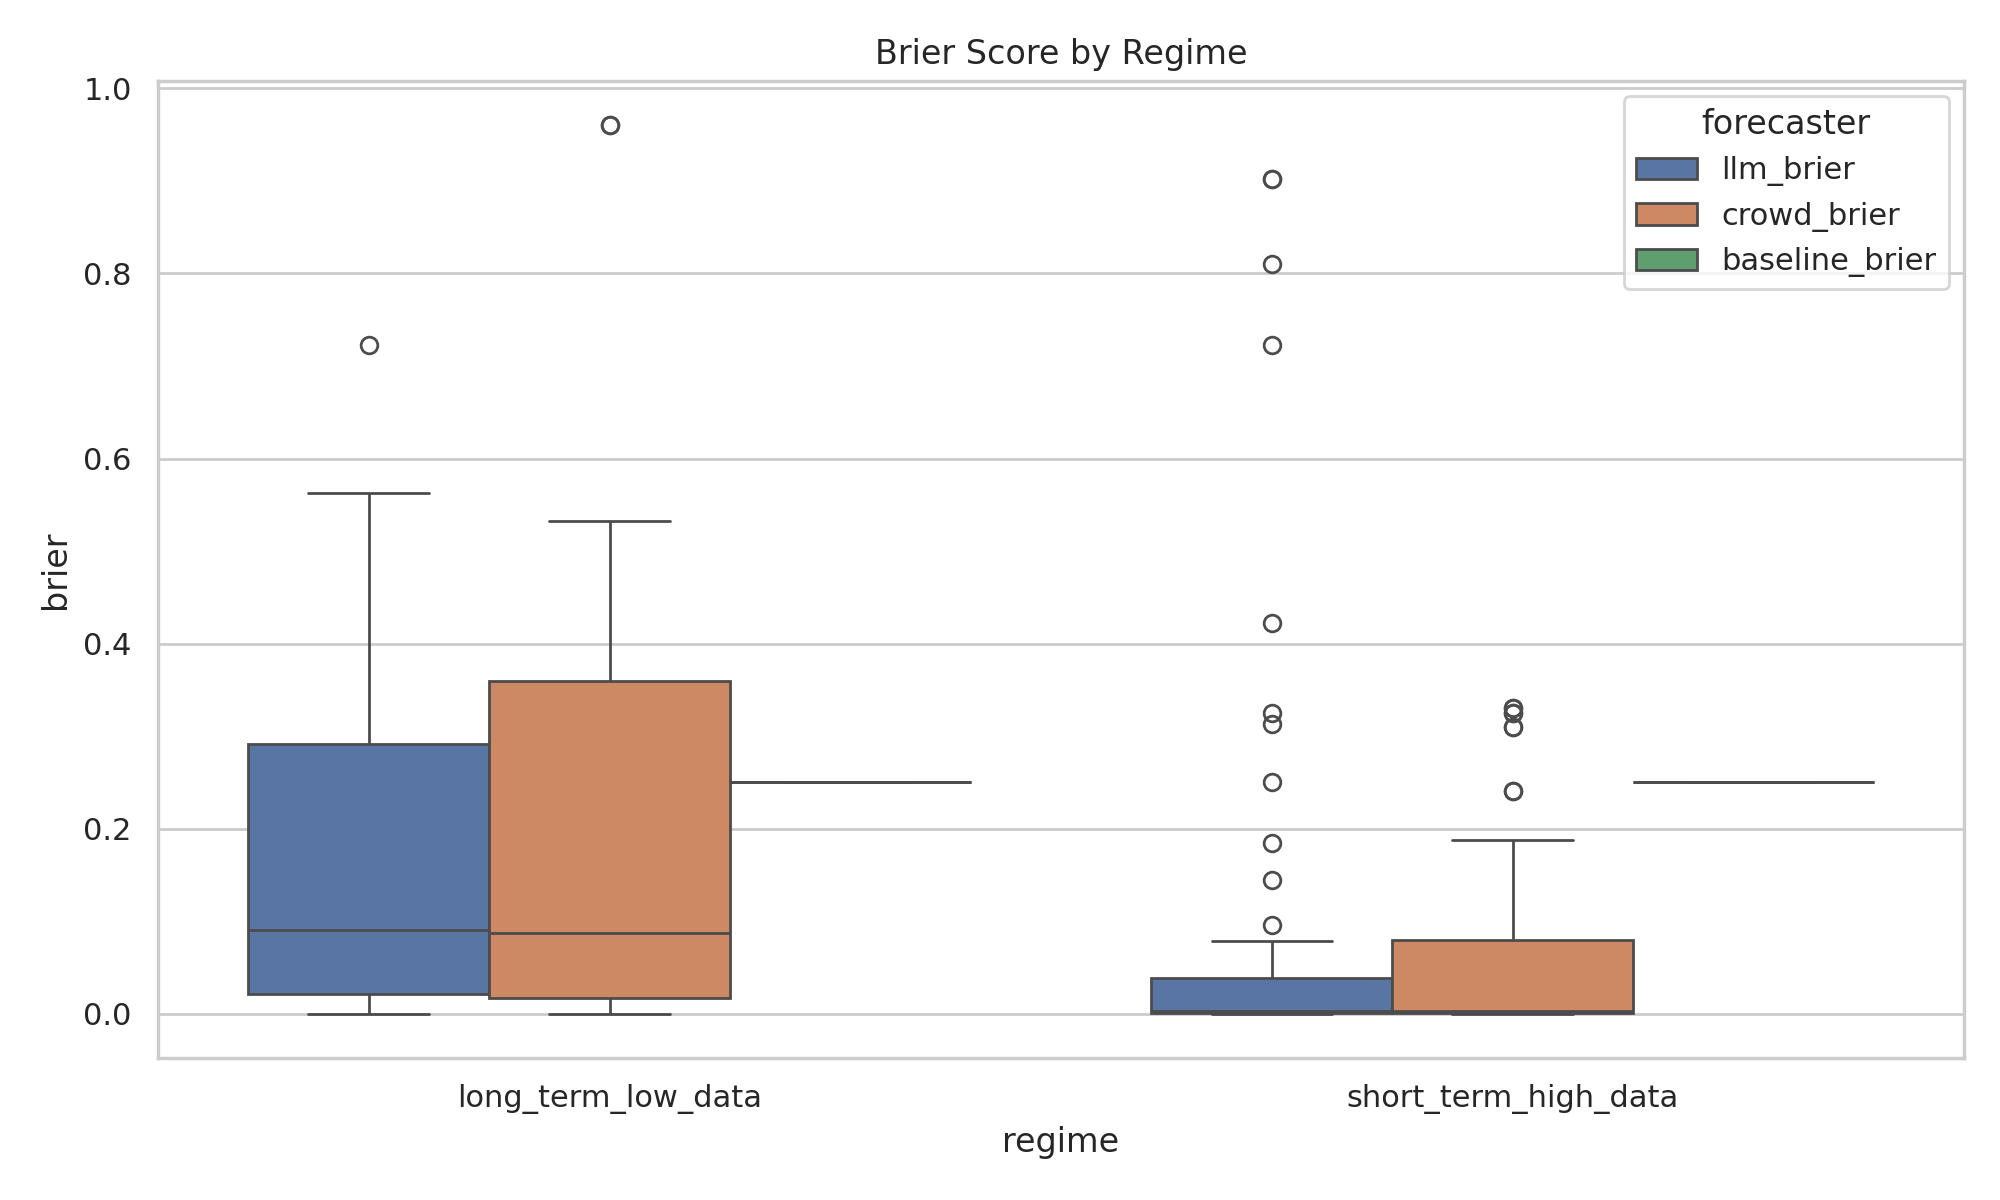
\includegraphics[width=0.95\linewidth]{figures/brier_by_regime.png}
    \caption{Mean \brier by regime and prompt condition. The \questiononly model performs best in \longterm, while the \withhistory condition is necessary to match or slightly beat the crowd in \shortterm.}
    \label{fig:brier_by_regime}
\end{figure}

\begin{figure}[t]
    \centering
    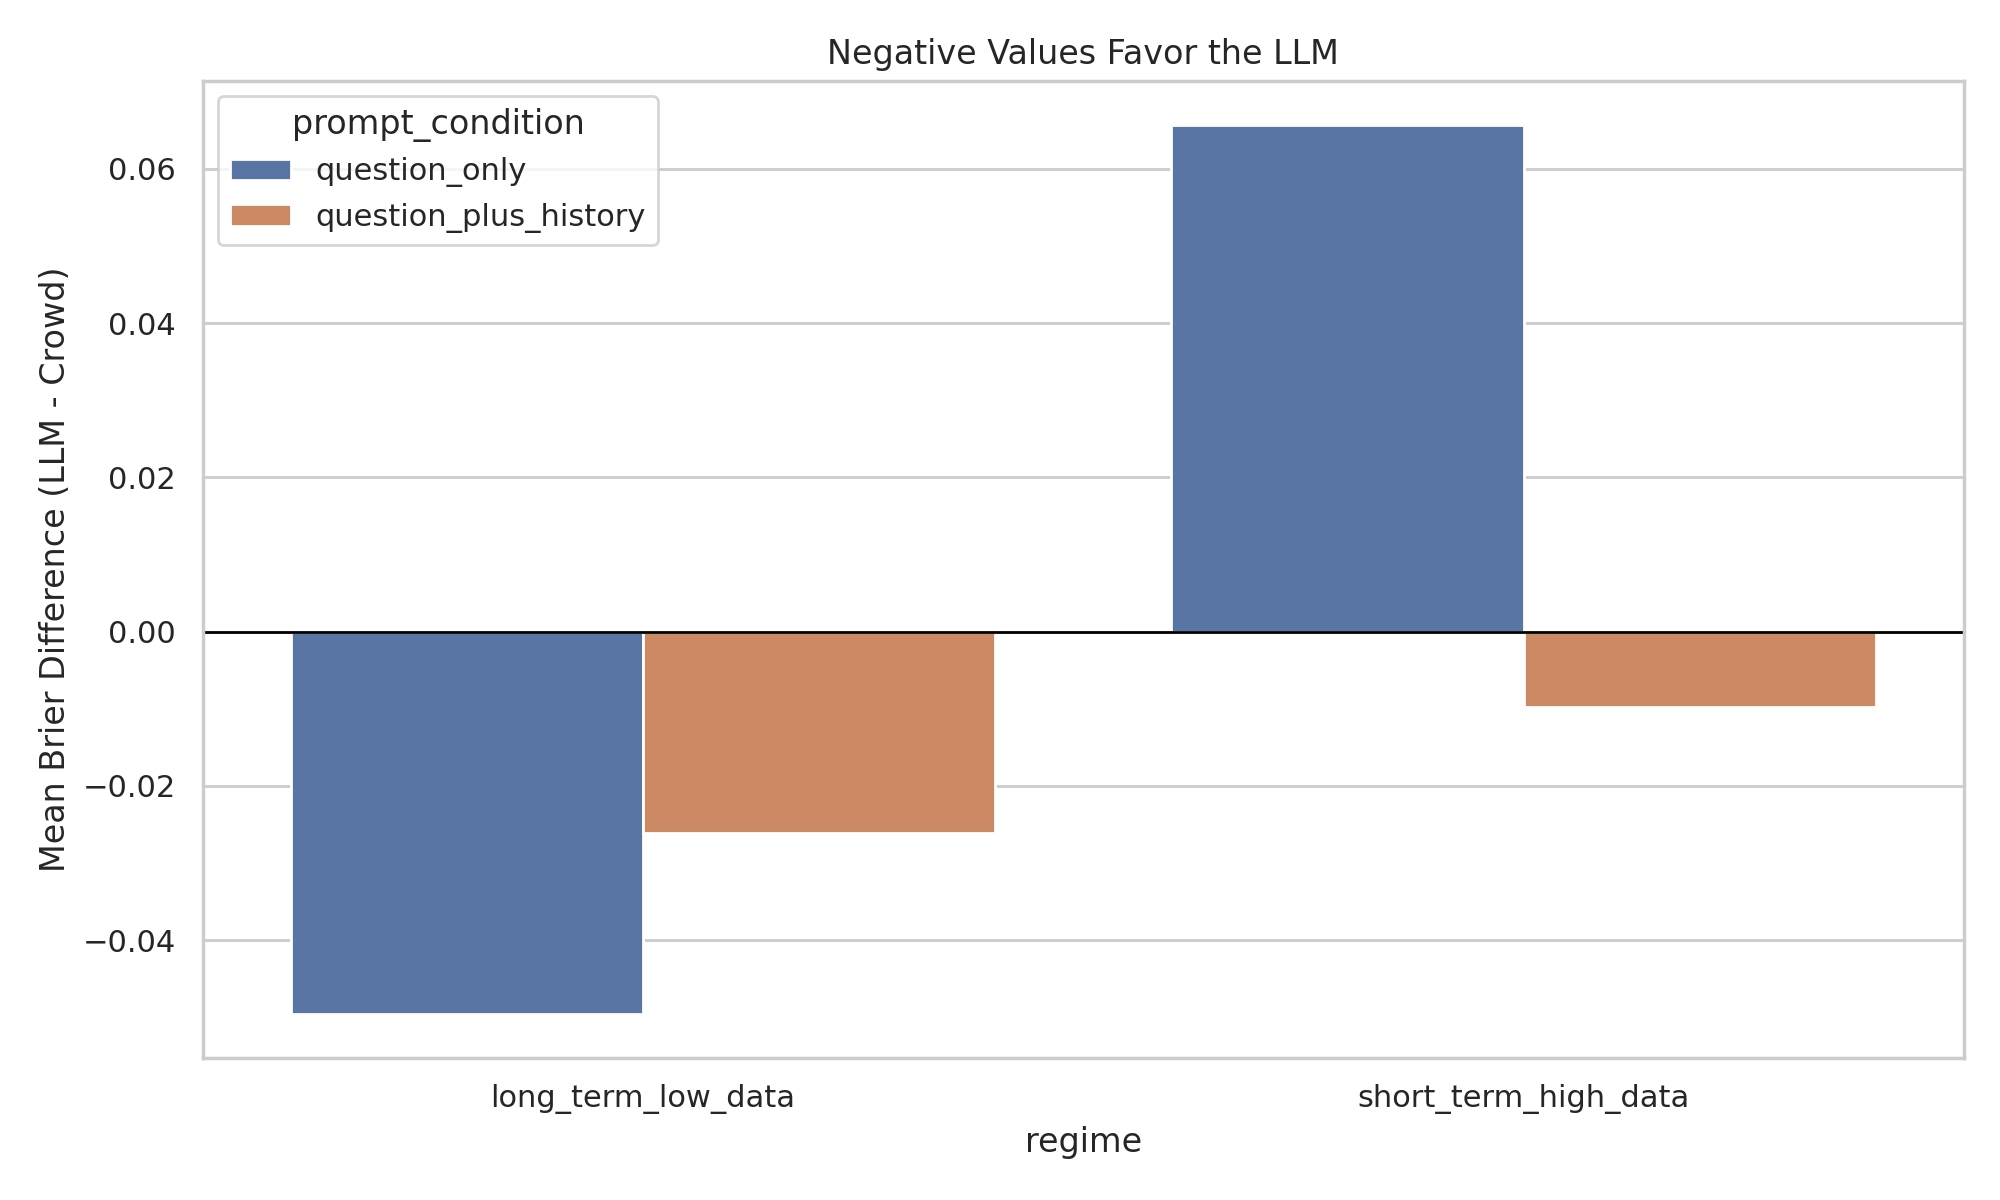
\includegraphics[width=0.95\linewidth]{figures/llm_minus_crowd_brier.png}
    \caption{Paired mean \brier difference $(\text{LLM} - \text{Crowd})$ by regime and prompt. Negative values favor the LLM. The sign flips across regimes for \questiononly, and history conditioning moves the short-horizon result close to parity.}
    \label{fig:llm_minus_crowd}
\end{figure}

\begin{figure}[t]
    \centering
    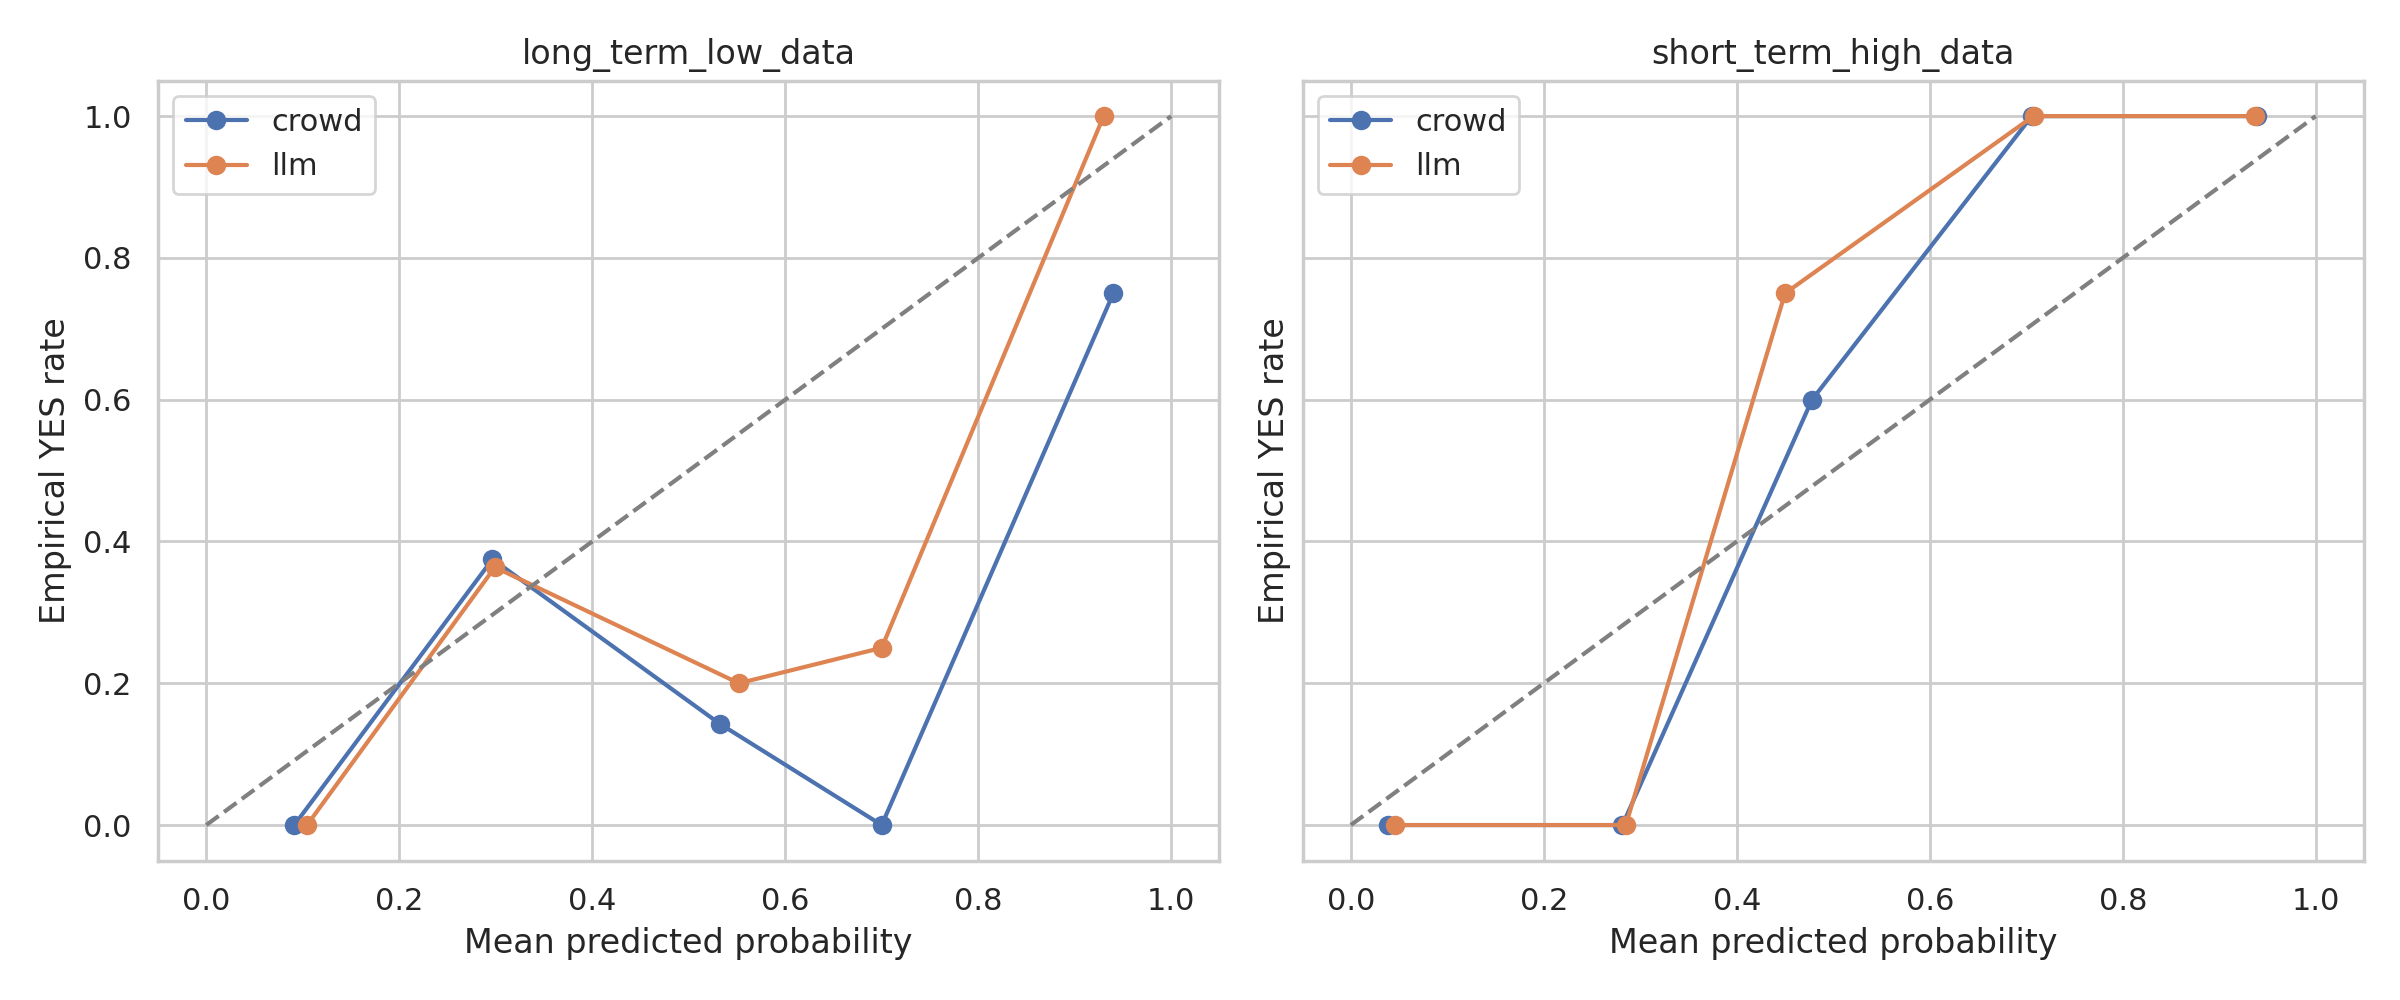
\includegraphics[width=0.95\linewidth]{figures/calibration_question_plus_history.png}
    \caption{Calibration under the \withhistory condition. The history-conditioned model is reasonably aligned overall, but the main improvement comes from correcting large short-horizon misses rather than from a uniform calibration gain across all bins.}
    \label{fig:calibration}
\end{figure}

\para{Error analysis.} The qualitative failures match the aggregate pattern. In \longterm, several extreme crowd probabilities on eventual NO outcomes create room for the LLM to win with more moderate forecasts. The report highlights a labor-force-participation question where the crowd assigned 0.98 to an outcome that resolved NO, while the LLM assigned 0.45 and incurred far less loss. A similar pattern appears on a Serbia/Kosovo conflict question, where the crowd was at 0.70 and the LLM at 0.18 before a NO resolution. In \shortterm without history, the opposite happens: the model stays near 0.05--0.15 on several eventual YES outcomes that the crowd had already updated toward, including a Biden impeachment inquiry and Spain winning the 2023 Women's World Cup. Those misses mostly disappear once the model sees the historical trajectory.

